\renewcommand{\leveltopI}{-11cm + \leveltop}
\renewcommand{\leveltopII}{-11cm + \leveltopI}
\renewcommand{\leveltopIII}{-11cm + \leveltopII}
\renewcommand{\leveltopIIII}{-10cm + \leveltopIII}
\renewcommand{\leveltopIIIII}{-10cm + \leveltopIIII}
\renewcommand{\leveltopIIIIII}{-10cm + \leveltopIIIII}
\renewcommand{\leveltopIIIIIII}{-10cm + \leveltopIIIIII}
\renewcommand{\leveltopIIIIIIII}{-9cm + \leveltopIIIIIII}
\renewcommand{\leveltopIIIIIIIII}{-8cm + \leveltopIIIIIIII}
\renewcommand{\leveltopIIIIIIIIII}{-7cm + \leveltopIIIIIIIII}
\begin{tikzpicture}[scale=.2, anchor=south, rotate=90]
\begin{scope}[yshift=\leveltopI cm, anchor = center]
\matrix (line1)[row sep=0.5cm] {
\node[draw=black, rectangle split,  rectangle split parts=3] (sn0x1c22990){
\footnotesize{100}
\nodepart{two}
\begin{tikzpicture}[scale=.2]
\node[circle, scale=0.75, fill] (tid0) at (4.5,1.5){};
\node[circle, scale=0.75, fill] (tid1) at (2.25,3){};
\node[circle, scale=0.75, fill] (tid4) at (0.75,4.5){};
\node[circle, scale=0.75, fill] (tid5) at (2.25,4.5){};
\node[circle, scale=0.75, fill] (tid6) at (3.75,4.5){};
\draw[](tid1) -- (tid4);
\draw[](tid1) -- (tid5);
\draw[](tid1) -- (tid6);
\node[circle, scale=0.75, fill] (tid2) at (6,3){};
\node[circle, scale=0.75, fill, task_scheduled] (tid7) at (5.25,4.5){};
\node[circle, scale=0.75, fill] (tid8) at (6.75,4.5){};
\draw[](tid2) -- (tid7);
\draw[](tid2) -- (tid8);
\node[circle, scale=0.75, fill] (tid3) at (8.25,3){};
\node[circle, scale=0.75, fill, task_scheduled] (tid9) at (8.25,4.5){};
\draw[](tid3) -- (tid9);
\draw[](tid0) -- (tid1);
\draw[](tid0) -- (tid2);
\draw[](tid0) -- (tid3);
\end{tikzpicture}
\nodepart{three}
\footnotesize{$50\:50$}
};
 \\ 
\\
};
\end{scope}
\begin{scope}[yshift=\leveltopII cm, anchor = center]
\matrix (line2)[row sep=0.5cm] {
\node[draw=black, rectangle split,  rectangle split parts=3] (sn0x1c29d30){
\footnotesize{50}
\nodepart{two}
\begin{tikzpicture}[scale=.2]
\node[circle, scale=0.75, fill] (tid0) at (4.5,1.5){};
\node[circle, scale=0.75, fill] (tid1) at (2.25,3){};
\node[circle, scale=0.75, fill, task_scheduled] (tid4) at (0.75,4.5){};
\node[circle, scale=0.75, fill] (tid5) at (2.25,4.5){};
\node[circle, scale=0.75, fill] (tid6) at (3.75,4.5){};
\draw[](tid1) -- (tid4);
\draw[](tid1) -- (tid5);
\draw[](tid1) -- (tid6);
\node[circle, scale=0.75, fill] (tid2) at (6,3){};
\node[circle, scale=0.75, fill, task_scheduled] (tid7) at (5.25,4.5){};
\node[circle, scale=0.75, fill] (tid8) at (6.75,4.5){};
\draw[](tid2) -- (tid7);
\draw[](tid2) -- (tid8);
\node[circle, scale=0.75, fill] (tid3) at (8.25,3){};
\draw[](tid0) -- (tid1);
\draw[](tid0) -- (tid2);
\draw[](tid0) -- (tid3);
\end{tikzpicture}
\nodepart{three}
\footnotesize{$50\:50$}
};
 \\ 
\node[draw=black, rectangle split,  rectangle split parts=3] (sn0x1c28c10){
\footnotesize{50}
\nodepart{two}
\begin{tikzpicture}[scale=.2]
\node[circle, scale=0.75, fill] (tid0) at (3.75,1.5){};
\node[circle, scale=0.75, fill] (tid1) at (2.25,3){};
\node[circle, scale=0.75, fill, task_scheduled] (tid4) at (0.75,4.5){};
\node[circle, scale=0.75, fill] (tid5) at (2.25,4.5){};
\node[circle, scale=0.75, fill] (tid6) at (3.75,4.5){};
\draw[](tid1) -- (tid4);
\draw[](tid1) -- (tid5);
\draw[](tid1) -- (tid6);
\node[circle, scale=0.75, fill] (tid2) at (5.25,3){};
\node[circle, scale=0.75, fill, task_scheduled] (tid7) at (5.25,4.5){};
\draw[](tid2) -- (tid7);
\node[circle, scale=0.75, fill] (tid3) at (6.75,3){};
\node[circle, scale=0.75, fill] (tid8) at (6.75,4.5){};
\draw[](tid3) -- (tid8);
\draw[](tid0) -- (tid1);
\draw[](tid0) -- (tid2);
\draw[](tid0) -- (tid3);
\end{tikzpicture}
\nodepart{three}
\footnotesize{$50\:50$}
};
 \\ 
\\
};
\end{scope}
\begin{scope}[yshift=\leveltopIII cm, anchor = center]
\matrix (line3)[row sep=0.5cm] {
\node[draw=black, rectangle split,  rectangle split parts=3] (sn0x1c29050){
\footnotesize{50}
\nodepart{two}
\begin{tikzpicture}[scale=.2]
\node[circle, scale=0.75, fill] (tid0) at (3.75,1.5){};
\node[circle, scale=0.75, fill] (tid1) at (2.25,3){};
\node[circle, scale=0.75, fill, task_scheduled] (tid4) at (0.75,4.5){};
\node[circle, scale=0.75, fill, task_scheduled] (tid5) at (2.25,4.5){};
\node[circle, scale=0.75, fill] (tid6) at (3.75,4.5){};
\draw[](tid1) -- (tid4);
\draw[](tid1) -- (tid5);
\draw[](tid1) -- (tid6);
\node[circle, scale=0.75, fill] (tid2) at (5.25,3){};
\node[circle, scale=0.75, fill] (tid7) at (5.25,4.5){};
\draw[](tid2) -- (tid7);
\node[circle, scale=0.75, fill] (tid3) at (6.75,3){};
\draw[](tid0) -- (tid1);
\draw[](tid0) -- (tid2);
\draw[](tid0) -- (tid3);
\end{tikzpicture}
\nodepart{three}
\footnotesize{$1$}
};
 \\ 
\node[draw=black, rectangle split,  rectangle split parts=3] (sn0x1c29fa0){
\footnotesize{25}
\nodepart{two}
\begin{tikzpicture}[scale=.2]
\node[circle, scale=0.75, fill] (tid0) at (3.75,1.5){};
\node[circle, scale=0.75, fill] (tid1) at (1.5,3){};
\node[circle, scale=0.75, fill, task_scheduled] (tid4) at (0.75,4.5){};
\node[circle, scale=0.75, fill] (tid5) at (2.25,4.5){};
\draw[](tid1) -- (tid4);
\draw[](tid1) -- (tid5);
\node[circle, scale=0.75, fill] (tid2) at (4.5,3){};
\node[circle, scale=0.75, fill, task_scheduled] (tid6) at (3.75,4.5){};
\node[circle, scale=0.75, fill] (tid7) at (5.25,4.5){};
\draw[](tid2) -- (tid6);
\draw[](tid2) -- (tid7);
\node[circle, scale=0.75, fill] (tid3) at (6.75,3){};
\draw[](tid0) -- (tid1);
\draw[](tid0) -- (tid2);
\draw[](tid0) -- (tid3);
\end{tikzpicture}
\nodepart{three}
\footnotesize{$50\:50$}
};
 \\ 
\node[draw=black, rectangle split,  rectangle split parts=3] (sn0x1c23690){
\footnotesize{25}
\nodepart{two}
\begin{tikzpicture}[scale=.2]
\node[circle, scale=0.75, fill] (tid0) at (3,1.5){};
\node[circle, scale=0.75, fill] (tid1) at (1.5,3){};
\node[circle, scale=0.75, fill, task_scheduled] (tid4) at (0.75,4.5){};
\node[circle, scale=0.75, fill] (tid5) at (2.25,4.5){};
\draw[](tid1) -- (tid4);
\draw[](tid1) -- (tid5);
\node[circle, scale=0.75, fill] (tid2) at (3.75,3){};
\node[circle, scale=0.75, fill, task_scheduled] (tid6) at (3.75,4.5){};
\draw[](tid2) -- (tid6);
\node[circle, scale=0.75, fill] (tid3) at (5.25,3){};
\node[circle, scale=0.75, fill] (tid7) at (5.25,4.5){};
\draw[](tid3) -- (tid7);
\draw[](tid0) -- (tid1);
\draw[](tid0) -- (tid2);
\draw[](tid0) -- (tid3);
\end{tikzpicture}
\nodepart{three}
\footnotesize{$50\:50$}
};
 \\ 
\\
};
\end{scope}
\begin{scope}[yshift=\leveltopIIII cm, anchor = center]
\matrix (line4)[row sep=0.5cm] {
\node[draw=black, rectangle split,  rectangle split parts=3] (sn0x1c23270){
\footnotesize{75}
\nodepart{two}
\begin{tikzpicture}[scale=.2]
\node[circle, scale=0.75, fill] (tid0) at (3,1.5){};
\node[circle, scale=0.75, fill] (tid1) at (1.5,3){};
\node[circle, scale=0.75, fill, task_scheduled] (tid4) at (0.75,4.5){};
\node[circle, scale=0.75, fill, task_scheduled] (tid5) at (2.25,4.5){};
\draw[](tid1) -- (tid4);
\draw[](tid1) -- (tid5);
\node[circle, scale=0.75, fill] (tid2) at (3.75,3){};
\node[circle, scale=0.75, fill] (tid6) at (3.75,4.5){};
\draw[](tid2) -- (tid6);
\node[circle, scale=0.75, fill] (tid3) at (5.25,3){};
\draw[](tid0) -- (tid1);
\draw[](tid0) -- (tid2);
\draw[](tid0) -- (tid3);
\end{tikzpicture}
\nodepart{three}
\footnotesize{$1$}
};
 \\ 
\node[draw=black, rectangle split,  rectangle split parts=3] (sn0x1c28250){
\footnotesize{12.5}
\nodepart{two}
\begin{tikzpicture}[scale=.2]
\node[circle, scale=0.75, fill] (tid0) at (3,1.5){};
\node[circle, scale=0.75, fill] (tid1) at (1.5,3){};
\node[circle, scale=0.75, fill, task_scheduled] (tid4) at (0.75,4.5){};
\node[circle, scale=0.75, fill] (tid5) at (2.25,4.5){};
\draw[](tid1) -- (tid4);
\draw[](tid1) -- (tid5);
\node[circle, scale=0.75, fill] (tid2) at (3.75,3){};
\node[circle, scale=0.75, fill, task_scheduled] (tid6) at (3.75,4.5){};
\draw[](tid2) -- (tid6);
\node[circle, scale=0.75, fill] (tid3) at (5.25,3){};
\draw[](tid0) -- (tid1);
\draw[](tid0) -- (tid2);
\draw[](tid0) -- (tid3);
\end{tikzpicture}
\nodepart{three}
\footnotesize{$50\:50$}
};
 \\ 
\node[draw=black, rectangle split,  rectangle split parts=3] (sn0x1c23860){
\footnotesize{12.5}
\nodepart{two}
\begin{tikzpicture}[scale=.2]
\node[circle, scale=0.75, fill] (tid0) at (2.25,1.5){};
\node[circle, scale=0.75, fill] (tid1) at (0.75,3){};
\node[circle, scale=0.75, fill, task_scheduled] (tid4) at (0.75,4.5){};
\draw[](tid1) -- (tid4);
\node[circle, scale=0.75, fill] (tid2) at (2.25,3){};
\node[circle, scale=0.75, fill, task_scheduled] (tid5) at (2.25,4.5){};
\draw[](tid2) -- (tid5);
\node[circle, scale=0.75, fill] (tid3) at (3.75,3){};
\node[circle, scale=0.75, fill] (tid6) at (3.75,4.5){};
\draw[](tid3) -- (tid6);
\draw[](tid0) -- (tid1);
\draw[](tid0) -- (tid2);
\draw[](tid0) -- (tid3);
\end{tikzpicture}
\nodepart{three}
\footnotesize{$1$}
};
 \\ 
\\
};
\end{scope}
\begin{scope}[yshift=\leveltopIIIII cm, anchor = center]
\matrix (line5)[row sep=0.5cm] {
\node[draw=black, rectangle split,  rectangle split parts=3] (sn0x1c285b0){
\footnotesize{6.25}
\nodepart{two}
\begin{tikzpicture}[scale=.2]
\node[circle, scale=0.75, fill] (tid0) at (3,1.5){};
\node[circle, scale=0.75, fill] (tid1) at (1.5,3){};
\node[circle, scale=0.75, fill, task_scheduled] (tid4) at (0.75,4.5){};
\node[circle, scale=0.75, fill, task_scheduled] (tid5) at (2.25,4.5){};
\draw[](tid1) -- (tid4);
\draw[](tid1) -- (tid5);
\node[circle, scale=0.75, fill] (tid2) at (3.75,3){};
\node[circle, scale=0.75, fill] (tid3) at (5.25,3){};
\draw[](tid0) -- (tid1);
\draw[](tid0) -- (tid2);
\draw[](tid0) -- (tid3);
\end{tikzpicture}
\nodepart{three}
\footnotesize{$1$}
};
 \\ 
\node[draw=black, rectangle split,  rectangle split parts=3] (sn0x1c23d40){
\footnotesize{93.75}
\nodepart{two}
\begin{tikzpicture}[scale=.2]
\node[circle, scale=0.75, fill] (tid0) at (2.25,1.5){};
\node[circle, scale=0.75, fill] (tid1) at (0.75,3){};
\node[circle, scale=0.75, fill, task_scheduled] (tid4) at (0.75,4.5){};
\draw[](tid1) -- (tid4);
\node[circle, scale=0.75, fill] (tid2) at (2.25,3){};
\node[circle, scale=0.75, fill, task_scheduled] (tid5) at (2.25,4.5){};
\draw[](tid2) -- (tid5);
\node[circle, scale=0.75, fill] (tid3) at (3.75,3){};
\draw[](tid0) -- (tid1);
\draw[](tid0) -- (tid2);
\draw[](tid0) -- (tid3);
\end{tikzpicture}
\nodepart{three}
\footnotesize{$1$}
};
 \\ 
\\
};
\end{scope}
\begin{scope}[yshift=\leveltopIIIIII cm, anchor = center]
\matrix (line6)[row sep=0.5cm] {
\node[draw=black, rectangle split,  rectangle split parts=3] (sn0x1c23fc0){
\footnotesize{100}
\nodepart{two}
\begin{tikzpicture}[scale=.2]
\node[circle, scale=0.75, fill] (tid0) at (2.25,1.5){};
\node[circle, scale=0.75, fill] (tid1) at (0.75,3){};
\node[circle, scale=0.75, fill, task_scheduled] (tid4) at (0.75,4.5){};
\draw[](tid1) -- (tid4);
\node[circle, scale=0.75, fill, task_scheduled] (tid2) at (2.25,3){};
\node[circle, scale=0.75, fill] (tid3) at (3.75,3){};
\draw[](tid0) -- (tid1);
\draw[](tid0) -- (tid2);
\draw[](tid0) -- (tid3);
\end{tikzpicture}
\nodepart{three}
\footnotesize{$50\:50$}
};
 \\ 
\\
};
\end{scope}
\begin{scope}[yshift=\leveltopIIIIIII cm, anchor = center]
\matrix (line7)[row sep=0.5cm] {
\node[draw=black, rectangle split,  rectangle split parts=3] (sn0x1c240d0){
\footnotesize{50}
\nodepart{two}
\begin{tikzpicture}[scale=.2]
\node[circle, scale=0.75, fill] (tid0) at (1.5,1.5){};
\node[circle, scale=0.75, fill] (tid1) at (0.75,3){};
\node[circle, scale=0.75, fill, task_scheduled] (tid3) at (0.75,4.5){};
\draw[](tid1) -- (tid3);
\node[circle, scale=0.75, fill, task_scheduled] (tid2) at (2.25,3){};
\draw[](tid0) -- (tid1);
\draw[](tid0) -- (tid2);
\end{tikzpicture}
\nodepart{three}
\footnotesize{$50\:50$}
};
 \\ 
\node[draw=black, rectangle split,  rectangle split parts=3] (sn0x1c241e0){
\footnotesize{50}
\nodepart{two}
\begin{tikzpicture}[scale=.2]
\node[circle, scale=0.75, fill] (tid0) at (2.25,1.5){};
\node[circle, scale=0.75, fill, task_scheduled] (tid1) at (0.75,3){};
\node[circle, scale=0.75, fill, task_scheduled] (tid2) at (2.25,3){};
\node[circle, scale=0.75, fill] (tid3) at (3.75,3){};
\draw[](tid0) -- (tid1);
\draw[](tid0) -- (tid2);
\draw[](tid0) -- (tid3);
\end{tikzpicture}
\nodepart{three}
\footnotesize{$1$}
};
 \\ 
\\
};
\end{scope}
\begin{scope}[yshift=\leveltopIIIIIIII cm, anchor = center]
\matrix (line8)[row sep=0.5cm] {
\node[draw=black, rectangle split,  rectangle split parts=3] (sn0x1c242f0){
\footnotesize{25}
\nodepart{two}
\begin{tikzpicture}[scale=.2]
\node[circle, scale=0.75, fill] (tid0) at (0.75,1.5){};
\node[circle, scale=0.75, fill] (tid1) at (0.75,3){};
\node[circle, scale=0.75, fill, task_scheduled] (tid2) at (0.75,4.5){};
\draw[](tid1) -- (tid2);
\draw[](tid0) -- (tid1);
\end{tikzpicture}
\nodepart{three}
\footnotesize{$1$}
};
 \\ 
\node[draw=black, rectangle split,  rectangle split parts=3] (sn0x1c245b0){
\footnotesize{75}
\nodepart{two}
\begin{tikzpicture}[scale=.2]
\node[circle, scale=0.75, fill] (tid0) at (1.5,1.5){};
\node[circle, scale=0.75, fill, task_scheduled] (tid1) at (0.75,3){};
\node[circle, scale=0.75, fill, task_scheduled] (tid2) at (2.25,3){};
\draw[](tid0) -- (tid1);
\draw[](tid0) -- (tid2);
\end{tikzpicture}
\nodepart{three}
\footnotesize{$1$}
};
 \\ 
\\
};
\end{scope}
\draw (sn0x1c22990.east) -- (sn0x1c28c10.west);
\draw (sn0x1c22990.east) -- (sn0x1c29d30.west);
\draw (sn0x1c29d30.east) -- (sn0x1c29fa0.west);
\draw (sn0x1c29d30.east) -- (sn0x1c29050.west);
\draw (sn0x1c28c10.east) -- (sn0x1c23690.west);
\draw (sn0x1c28c10.east) -- (sn0x1c29050.west);
\draw (sn0x1c29050.east) -- (sn0x1c23270.west);
\draw (sn0x1c29fa0.east) -- (sn0x1c28250.west);
\draw (sn0x1c29fa0.east) -- (sn0x1c23270.west);
\draw (sn0x1c23690.east) -- (sn0x1c23860.west);
\draw (sn0x1c23690.east) -- (sn0x1c23270.west);
\draw (sn0x1c23270.east) -- (sn0x1c23d40.west);
\draw (sn0x1c28250.east) -- (sn0x1c23d40.west);
\draw (sn0x1c28250.east) -- (sn0x1c285b0.west);
\draw (sn0x1c23860.east) -- (sn0x1c23d40.west);
\draw (sn0x1c285b0.east) -- (sn0x1c23fc0.west);
\draw (sn0x1c23d40.east) -- (sn0x1c23fc0.west);
\draw (sn0x1c23fc0.east) -- (sn0x1c240d0.west);
\draw (sn0x1c23fc0.east) -- (sn0x1c241e0.west);
\draw (sn0x1c240d0.east) -- (sn0x1c242f0.west);
\draw (sn0x1c240d0.east) -- (sn0x1c245b0.west);
\draw (sn0x1c241e0.east) -- (sn0x1c245b0.west);
\end{tikzpicture}
%% profile
\begin{tikzpicture}[scale=.2, anchor=south, rotate=90]
\begin{scope}[yshift=\leveltopI cm, anchor = center]
\matrix (line1)[row sep=0.1cm] {
\node[draw=black, rectangle split,  rectangle split parts=3] (sn0x1c22990){
\footnotesize{100}
\nodepart{two}
\begin{tikzpicture}[scale=.2]
\node[rectangle, scale=0.75] at (0, 0) {$\profile{6, 3, 1}$};
\end{tikzpicture}
\nodepart{three}
\footnotesize{$1$}
};
 \\ 
\\
};
\end{scope}
\begin{scope}[yshift=\leveltopII cm, anchor = center]
\matrix (line2)[row sep=0.1cm] {
\node[draw=black, rectangle split,  rectangle split parts=3] (sn0x1c28c10){
\footnotesize{100}
\nodepart{two}
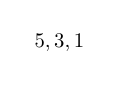
\begin{tikzpicture}[scale=.2]
\node[rectangle, scale=0.75] at (0, 0) {$\profile{5, 3, 1}$};
\end{tikzpicture}
\nodepart{three}
\footnotesize{$1$}
};
 \\ 
\\
};
\end{scope}
\begin{scope}[yshift=\leveltopIII cm, anchor = center]
\matrix (line3)[row sep=0.1cm] {
\node[draw=black, rectangle split,  rectangle split parts=3] (sn0x1c29fa0){
\footnotesize{100}
\nodepart{two}
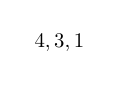
\begin{tikzpicture}[scale=.2]
\node[rectangle, scale=0.75] at (0, 0) {$\profile{4, 3, 1}$};
\end{tikzpicture}
\nodepart{three}
\footnotesize{$1$}
};
 \\ 
\\
};
\end{scope}
\begin{scope}[yshift=\leveltopIIII cm, anchor = center]
\matrix (line4)[row sep=0.1cm] {
\node[draw=black, rectangle split,  rectangle split parts=3] (sn0x1c28250){
\footnotesize{100}
\nodepart{two}
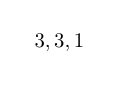
\begin{tikzpicture}[scale=.2]
\node[rectangle, scale=0.75] at (0, 0) {$\profile{3, 3, 1}$};
\end{tikzpicture}
\nodepart{three}
\footnotesize{$1$}
};
 \\ 
\\
};
\end{scope}
\begin{scope}[yshift=\leveltopIIIII cm, anchor = center]
\matrix (line5)[row sep=0.1cm] {
\node[draw=black, rectangle split,  rectangle split parts=3] (sn0x1c23d40){
\footnotesize{100}
\nodepart{two}
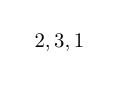
\begin{tikzpicture}[scale=.2]
\node[rectangle, scale=0.75] at (0, 0) {$\profile{2, 3, 1}$};
\end{tikzpicture}
\nodepart{three}
\footnotesize{$1$}
};
 \\ 
\\
};
\end{scope}
\begin{scope}[yshift=\leveltopIIIIII cm, anchor = center]
\matrix (line6)[row sep=0.1cm] {
\node[draw=black, rectangle split,  rectangle split parts=3] (sn0x1c23fc0){
\footnotesize{100}
\nodepart{two}
\begin{tikzpicture}[scale=.2]
\node[rectangle, scale=0.75] at (0, 0) {$\profile{1, 3, 1}$};
\end{tikzpicture}
\nodepart{three}
\footnotesize{$50\:50$}
};
 \\ 
\\
};
\end{scope}
\begin{scope}[yshift=\leveltopIIIIIII cm, anchor = center]
\matrix (line7)[row sep=0.1cm] {
\node[draw=black, rectangle split,  rectangle split parts=3] (sn0x1c240d0){
\footnotesize{50}
\nodepart{two}
\begin{tikzpicture}[scale=.2]
\node[rectangle, scale=0.75] at (0, 0) {$\profile{1, 2, 1}$};
\end{tikzpicture}
\nodepart{three}
\footnotesize{$50\:50$}
};
 \\ 
\node[draw=black, rectangle split,  rectangle split parts=3] (sn0x1c241e0){
\footnotesize{50}
\nodepart{two}
\begin{tikzpicture}[scale=.2]
\node[rectangle, scale=0.75] at (0, 0) {$\profile{3, 1}$};
\end{tikzpicture}
\nodepart{three}
\footnotesize{$1$}
};
 \\ 
\\
};
\end{scope}
\begin{scope}[yshift=\leveltopIIIIIIII cm, anchor = center]
\matrix (line8)[row sep=0.1cm] {
\node[draw=black, rectangle split,  rectangle split parts=3] (sn0x1c242f0){
\footnotesize{25}
\nodepart{two}
\begin{tikzpicture}[scale=.2]
\node[rectangle, scale=0.75] at (0, 0) {$\profile{1, 1, 1}$};
\end{tikzpicture}
\nodepart{three}
\footnotesize{$1$}
};
 \\ 
\node[draw=black, rectangle split,  rectangle split parts=3] (sn0x1c245b0){
\footnotesize{75}
\nodepart{two}
\begin{tikzpicture}[scale=.2]
\node[rectangle, scale=0.75] at (0, 0) {$\profile{2, 1}$};
\end{tikzpicture}
\nodepart{three}
\footnotesize{$1$}
};
 \\ 
\\
};
\end{scope}
\draw (sn0x1c22990.east) -- (sn0x1c28c10.west);
\draw (sn0x1c28c10.east) -- (sn0x1c29fa0.west);
\draw (sn0x1c29fa0.east) -- (sn0x1c28250.west);
\draw (sn0x1c28250.east) -- (sn0x1c23d40.west);
\draw (sn0x1c23d40.east) -- (sn0x1c23fc0.west);
\draw (sn0x1c23fc0.east) -- (sn0x1c240d0.west);
\draw (sn0x1c23fc0.east) -- (sn0x1c241e0.west);
\draw (sn0x1c240d0.east) -- (sn0x1c242f0.west);
\draw (sn0x1c240d0.east) -- (sn0x1c245b0.west);
\draw (sn0x1c241e0.east) -- (sn0x1c245b0.west);
\end{tikzpicture}
%%% Local Variables:
%%% TeX-master: "../thesis.tex"
%%% End: 